\subsection{BÀI TẬP TRẮC NGHIỆM}
\Opensolutionfile{ans}[ans/ans0D6-B1]

\begin{ex}%[0D2Y1-1]
	Điểm nào sau đây thuộc đồ thị hàm số $y = 2x^2 + x - 3$?
	\choice
	{\True $\left(0;-3\right)$}
	{$\left(-2;1\right)$}
	{$\left(-1;0\right)$}
	{$\left(3;-7\right)$}
	\loigiai{Thử tọa độ các điểm vào hàm số ta được điểm $\left(0;-3\right)$ thuộc đồ thị hàm số.
	}
\end{ex}


\begin{ex}%[0D2Y1]
	Điểm nào sau đây thuộc đồ thị hàm số  $y=3x^3-2x+1$?
	\choice
	{$\left( -1;2 \right)$}
	{$\left( 1;1 \right)$}
	{$\left( 0;0 \right)$}
	{\True  $\left( 1;2 \right)$}
	\loigiai
	{\begin{itemize}
			\item Với $ x = -1 \Rightarrow y = 0 $ nên $ (-1;2) $ không thuộc đồ thị hàm số $y=3x^3-2x+1$.
			\item Với $ x = 1 \Rightarrow y = 2 $ nên $ (1;2) $ thuộc đồ thị hàm số $y=3x^3-2x+1$.
		\end{itemize}
	}
\end{ex}

\begin{ex}%[0D2B1]
	Tìm tập xác định $\mathcal{D}$ của hàm số $y=\dfrac{x-1}{x-2}$.
	\choice
	{\True $\mathcal{D}=\mathbb{R}\setminus\{2\}$}
	{$\mathcal{D}=\mathbb{R}\setminus\{1\}$}
	{$\mathcal{D}=\mathbb{R}$}
	{$\mathcal{D}=\mathbb{R}\setminus\{1;2\}$}
	\loigiai{
		\begin{itemize}
			\item [$\bullet$] Điều kiện xác định $x-2 \ne 0 \Leftrightarrow x \ne 2$.
			\item [$\bullet$] Suy ra, tập xác định là $\mathcal{D}=\mathbb{R}\setminus\{2\}$.
		\end{itemize}
	}
\end{ex}

\begin{ex}%[0D2B1]
	Tìm tập xác định $\mathcal{D}$ của hàm số $y=\dfrac{x-2}{x^2-2x+2}$.
	\choice
	{$\mathcal{D}=\mathbb{R}\setminus\{1\}$}
	{$\mathcal{D}=\mathbb{R}\setminus\{2\}$}
	{\True $\mathcal{D}=\mathbb{R}$}
	{$\mathcal{D}=\mathbb{R}\setminus\{1;2\}$}
	\loigiai{
		\begin{itemize}
			\item [$\bullet$] Điều kiện xác định $x^2-2x+2 \ne 0$ (luôn đúng).
			\item [$\bullet$] Suy ra, tập xác định là $\mathcal{D}=\mathbb{R}$.
		\end{itemize}
	}
\end{ex}

\begin{ex}%[0D2B1]
	Tìm tập xác định $\mathcal{D}$ của hàm số $y=\sqrt{x-2}$.
	\choice
	{$\mathcal{D}=\mathbb{R}\setminus\{2\}$}
	{$\mathcal{D}=(2;+\infty)$}
	{$\mathcal{D}=(-\infty;2)$}
	{\True $\mathcal{D}=[2;+\infty)$}
	\loigiai{
		\begin{itemize}
			\item [$\bullet$] Điều kiện xác định $x-2 \ge 0 \Leftrightarrow x \ge 2$.
			\item [$\bullet$] Suy ra, tập xác định là $\mathcal{D}=[2;+\infty)$.
		\end{itemize}
	}
\end{ex}

\begin{ex}%[0D2B1]
	Tìm tập xác định của hàm số $y=\dfrac{2x+3}{x^2-x}$.
	\choice{$\mathbb{R}\setminus\{1\}$}
	{$\mathbb{R}$}
	{$\mathbb{R}\setminus\{0\}$}
	{\True $\mathbb{R}\setminus\{0,1\}$}
	\loigiai{
			\begin{itemize}
				\item [$\bullet$] Điều kiện xác định $x^2-x \ne 0 \Leftrightarrow x \ne 0$ và $x \ne 1$.
				\item [$\bullet$] Suy ra, tập xác định là $\mathcal{D}=\mathbb{R}\setminus\{0,1\}$.
			\end{itemize}
	}
\end{ex}

\begin{ex}%[0D2B1-3]%
	\immini{Cho hàm số $y=f(x)$ có tập xác định là $[-3;3]$ và đồ thị của nó được biểu diễn bởi hình bên. Khẳng định nào sau đây đúng?
	\choice
	{\True Hàm số đồng biến trên khoảng $(-3;-1)$}
	{Hàm số đồng biến trên khoảng $(-3;3)$}
	{Hàm số đồng biến trên khoảng $(-3;0)$}
	{Hàm số nghịch biến trên khoảng $(-1;2)$}}{
	\begin{tikzpicture}[>=stealth,x=1.0 cm,y=1.0 cm, scale=0.75]
		\draw[->] (-3.5,0)--(4,0) node[below left] {$x$};
		\draw[->] (0,-2)--(0,4.5) node[below right] {$y$};
		\foreach \x in {,-3,-2,-1,1,2,3,,}
		\draw[shift={(\x,0)},color=black] (0pt,2pt) -- (0pt,-2pt) node[below] {\footnotesize $\x$};
		\foreach \y in {,-1,1,2,3,4,}
		\draw[shift={(0,\y)},color=black] (2pt,0pt) -- (-2pt,0pt) node[left] {\footnotesize $\y$};
		\draw[color=black] (0pt,-10pt) node[right] {\footnotesize $0$};
		\clip(-4,-2.5) rectangle (4,4.5);
		\draw[dashed] (0,-1)--(-3,-1)--(-3,0);
		\draw[dashed] (-1,0)--(-1,1)--(0,1);
		\draw[dashed] (0,4)--(3,4)--(3,0);
		\draw[magenta,thick] (-3,-1)--(-1,1)--(0,1)--(3,4);
\end{tikzpicture}}
	\loigiai{
		Trên khoảng $(-3;-1)$ và $(1;3)$, đồ thị hàm số đi lên, do đó hàm số đồng biến trên $(-3;-1)$ và $(1;3)$.
	}
\end{ex}

\begin{ex}%[0D2B1-3]%
	Khẳng định nào sau đây về hàm số $y=x^2$ là khẳng định đúng?
	\choice
	{Hàm số nghịch biến trên $\mathbb{R}$}
	{Hàm số đồng biến trên $\mathbb{R}$}
	{Hàm số nghịch biến trên $[0;+\infty)$}
	{\True Hàm số đồng biến trên $[0;+\infty)$}
	\loigiai{
		Hàm số $y=x^2$ có hệ số $a=1>0$ nên hàm đồng biến trên $\left(-\dfrac{b}{2a};+\infty \right) $ hay  $[0;+\infty)$ (vì hàm số chỉ bằng $0$ tại một điểm là $x=0$).
	}
\end{ex}

\begin{ex}
	\immini{Cho hàm số $y=f(x)$ liên tục trên $\mathbb{R}$ và có đồ thị như hình bên. Khẳng định nào sau đây đúng?
	\choice
		{Hàm số đồng biến trên khoảng $(1;3)$}
		{Hàm số nghịch biến trên khoảng $(6;+\infty)$}
		{Hàm số đồng biến trên khoảng $(-\infty;3)$}
		{\True Hàm số nghịch biến trên khoảng $(3;6)$}
	}{
		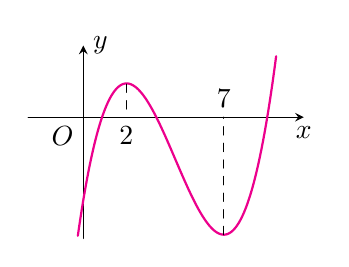
\begin{tikzpicture}[>=stealth,line cap=round,line join=round,x=1cm,y=1cm,scale=0.7]
			\draw[->] (-1,0)--(4,0) node[below] {$x$};
			\draw[->] (0,-2.2)--(0,1.3) node[right] {$y$};
			\node[below left](0,0){$O$};
			\draw[magenta,thick,samples=1000,domain=-0.1:3.5] plot(\x,{(\x-1)^3-2*(\x-1)^2-(\x)+1.5});
			\draw[dashed] (0.78,0.6) -- (0.78,0) node[below] {$2$};
			\draw[dashed] (2.55,-2.13) -- (2.55,0) node[above] {$7$};
	\end{tikzpicture}}
	\loigiai{
		Dựa vào đồ thị thấy hàm số nghịch biến trên khoảng $(2;7)$, do đó hàm số nghịch biến trên khoảng $(3;6)$.
	}
\end{ex}

\begin{ex}%[0D2Y1]
	Tập xác định của hàm số $y=\dfrac{x^2+\sqrt{3-x}}{x-2}$ là
	\choice
	{$(-\infty;3)\backslash \{2\}$}
	{$(2;3]$}
	{\True $(-\infty;3]\backslash \{2\}$}
	{$(-\infty;3]$}
	\loigiai{
		\begin{itemize}
			\item [$\bullet$] Điều kiện xác định $\heva{& 3-x \ge 0\\&x-2 \ne 0} \Leftrightarrow \heva{& x \le 3\\&x \ne 2}$.
			\item [$\bullet$] Suy ra, tập xác định là $\mathcal{D}=(-\infty;3]\backslash \{2\}$.
		\end{itemize}
	}
\end{ex}

\begin{ex}%[0D2B1]
	Tìm tập xác định của hàm số $y=\sqrt{3+x}+\sqrt{6-x}$.
	\choice
	{\True $[-3;6]$}
	{$(-3;6)$}
	{$(-\infty;-3)\cup (6;+\infty)$}
	{$\mathbb{R}\backslash(-3;6)$}
	\loigiai{
		\begin{itemize}
			\item [$\bullet$] Điều kiện xác định $\heva{& 3+x \ge 0\\& 6-x \ge 0} \Leftrightarrow -3\le x\le 6$.
			\item [$\bullet$] Suy ra, tập xác định là $\mathscr{D}=[-3;6]$.
		\end{itemize}
	}
\end{ex}

\begin{ex}%[0D2B1-2]
	Tập xác định của hàm số $y=\dfrac{x+2}{\sqrt{x-1}}+\sqrt{3-x}$ là
	\choice
	{$[1;3]$}
	{\True $(1;3]$}
	{$(-\infty;3]$}
	{$(1;+\infty)$}
	\loigiai{
		$$\dfrac{x+2}{\sqrt{x-1}}+\sqrt{3-x}\text{ có nghĩa }\Leftrightarrow \heva{&x-1>0\\&3-x\geq 0}\Leftrightarrow 1<x\leq 3.$$
		Vậy tập xác định của hàm số đã cho là $(1;3]$.
	}
\end{ex}

\begin{ex}
	\immini{Cho hàm số $y=f(x)$ liên tục trên $\mathbb{R}$ và có đồ thị như hình bên. Tính giá trị biểu thức $P=2f(1)+f(4)-f(3)$
		\haicot
		{$P=1$}
		{$P=0$}
		{\True $P=2$}
		{$P=4$}
	}{\hspace{1cm}
		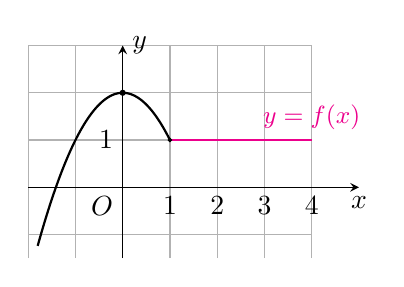
\begin{tikzpicture}[smooth,samples=300,scale=0.6,>=stealth]
		\draw[black!30!] (-2,-1.5) grid (4,3);
		\draw[->] (-2,0)--(5,0) node[below]{$x$};
		\draw[->] (0,-1.5)--(0,3) node[right]{$y$};
		\foreach \x in {1,2,3,4}{
			\draw (\x,0) node[below]{$\x$};%Ox
		}
		\foreach \y in {1}{
			\draw (0,\y) node[left]{$\y$};%Oy
		}
		\draw (0,0) node[below left]{$O$};
		\draw[domain=-1.8:1,thick] plot(\x,{-(\x)^2+2});
		\draw [magenta,thick](1,1)--(4,1) node[above]{\small $y=f(x)$};
		\draw[fill=black] (0,2) circle(1.5pt) (1,1) circle(1pt);
		\end{tikzpicture}}
		\loigiai{
		Quan sát đồ thị, ta có các kết quả $f(1)=1$, $f(3)=1$ và $f(4)=1$ nên
		$$P=2f(1)+f(4)-f(3)=2+1-1=2.$$
	}
\end{ex}
\begin{ex}%[0D2Y1-1]
	Cho hàm số $y=f(x)=\heva{&\sqrt{x+4}&&\text{ khi } x>1\\&x^2+1&&\text{ khi } -1\leq x\leq 1\\&2x-1&&\text{ khi } x<-1}$. Giá trị $f(0)$ bằng
	\choice
	{$-2$}
	{$2$}
	{$-1$}
	{\True $1$}
	\loigiai{
		Ta có $f(0)=0^2+1=1$.
	}
\end{ex}

\begin{ex}%[0D2Y1-1]
	Cho hàm số $y=\heva{&2x+1 &\text{khi}\ x\le 2\\ &x^2-3 &\text{khi}\ x>2}$. Trong các điểm sau đây, điểm nào thuộc đồ thị hàm số?
	\choice
	{\True $(0;1)$}
	{$(0;-3)$}
	{$(3;7)$}
	{$(-3;6)$}
	\loigiai{
		Điểm $(0;1)$ thuộc đồ thị hàm số.
	}
\end{ex}

\begin{ex}
	\immini{Cho đồ thị hàm số $y=f(x)$ trên miền $[-3;5]$ như hình bên. Trong các điểm sau, điểm nào thuộc đồ thị hàm số đã cho?
	\haicot
	{$A(4;1)$}
	{$B(1;1)$ }
	{\True $C(3;3)$}
	{$D(0;2)$ }}{
	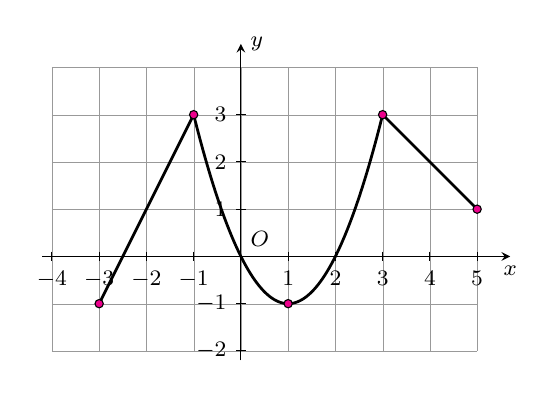
\begin{tikzpicture}[smooth,samples=300,scale=0.6,>=stealth,font=\footnotesize]
		\draw[line width=0.1pt,gray!80] (-4,-2) grid (5,4);
		\draw[->] (-4.2,0)--(5.7,0) node[below]{$x$};
		\draw[->] (0,-2.2)--(0,4.5) node[right]{$y$};
		\draw (0,0) node[above right]{$O$};
		\draw[line width=1pt,domain=-1:3] plot(\x,{(\x-1)^2-1});
		\draw[line width=1pt] (-3,-1)--(-1,3) (3,3)--(5,1);
		\draw[fill=magenta] (-3,-1) circle(2.5pt) (-1,3) circle(2.5pt) (3,3) circle(2.5pt) (5,1) circle(2.5pt) (1,-1) circle(2.5pt);
		\foreach \x in {-4,-3,-2,-1,1,2,3,4,5}\draw (\x,0.1)--(\x,-0.1) node [below] {\footnotesize $\x$};
		\foreach \y in {-2,-1,1,2,3}\draw (0.1,\y)--(-0.1,\y) node [left] {\footnotesize $\y$};
\end{tikzpicture}}
\loigiai{}
\end{ex}

\begin{ex}
	\immini{Cho đồ thị hàm số $y=f(x)$ trên miền $\mathscr{D}=[-3;5]$ như hình bên. Tập giá trị của hàm số này trên miền $\mathscr{D}$ là
		\haicot
		{$[-3;5]$}
		{$[-2;5]$ }
		{$[-3;3]$}
		{\True $[-2;2]$}}{
		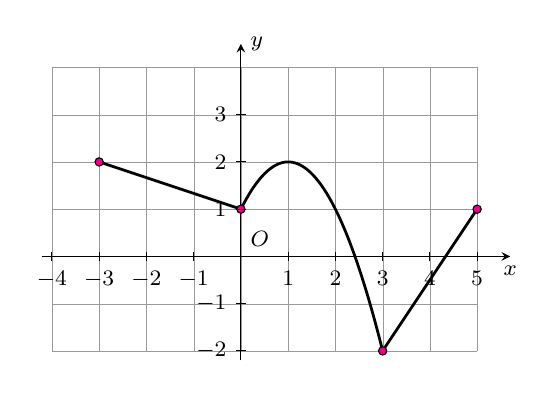
\begin{tikzpicture}[smooth,samples=300,scale=0.6,>=stealth,font=\footnotesize]
			\draw[line width=0.1pt,gray!80] (-4,-2) grid (5,4);
			\draw[->] (-4.2,0)--(5.7,0) node[below]{$x$};
			\draw[->] (0,-2.2)--(0,4.5) node[right]{$y$};
			\draw (0,0) node[above right]{$O$};
			\draw[line width=1pt,domain=0:3] plot(\x,{-(\x-1)^2+2});
			\draw[line width=1pt] (-3,2)--(0,1) (3,-2)--(5,1);
			\draw[fill=magenta] (-3,2) circle(2.5pt) (0,1) circle(2.5pt) (3,-2) circle(2.5pt) (5,1) circle(2.5pt) ;
			\foreach \x in {-4,-3,-2,-1,1,2,3,4,5}\draw (\x,0.1)--(\x,-0.1) node [below] {\footnotesize $\x$};
			\foreach \y in {-2,-1,1,2,3}\draw (0.1,\y)--(-0.1,\y) node [left] {\footnotesize $\y$};
	\end{tikzpicture}}
	\loigiai{}
\end{ex}


\begin{ex}%[0D2B1]
	Cho hàm số $y=\dfrac{x+1}{x-1}$. Tìm tọa độ điểm thuộc đồ thị của hàm số có tung độ bằng $-2$.
	\choice        
	{$(0;-2)$}
	{\True $\left(\dfrac{1}{3};-2\right)$}
	{$(-2;-2)$}
	{$(-1;-2)$}
	\loigiai{
		Thay $y=-2$ vào phương trình hàm số $y=\dfrac{x+1}{x-1}$ ta được $x=\dfrac{1}{3}$.
	}
\end{ex}
\begin{ex}%[Phan Anh]%[0D2B1-1]
	Điểm nào sau đây thuộc đồ thị hàm số $y=\dfrac{1}{x-1}$?
	\choice
	{\True $M_1(2;1)$}
	{$M_2(1;1)$}
	{$M_3(2;0)$}
	{$M_4(0;-2)$}
	\loigiai{
		Xét điểm $M_1$, thay $x=2$ và $y=1$
		vào hàm số $y=\dfrac{1}{x-1}$ ta được $1=\dfrac{1}{2-1}$ ta thấy đúng nên nhận $M_1$.}
\end{ex}
\begin{ex}%[Phan Anh]%[0D2B1-1]
	Điểm nào sau đây \textbf{không} thuộc đồ thị hàm số $y=\dfrac{\sqrt{x^2-4x+4}}{x}$?
	\choice
	{$A\left(2;0\right)$}
	{$B\left(3;\dfrac{1}{3}\right)$}
	{\True $C\left(1;-1\right)$}
	{$D\left(-1;-3\right)$}
	\loigiai{Thay từng đáp án vào hàm số $y=\dfrac{\sqrt{x^2-4x+4}}{x}$.
		\begin{itemize}
			\item Với $x=2$ và $y=0$, ta được $0=\dfrac{\sqrt{2^2-4.2+4}}{2}$ (đúng).
			\item Với $x=3$ và $y=\dfrac{1}{3}$, ta được $\dfrac{1}{3}=\dfrac{\sqrt{3^2-4\cdot3+4}}{3}$ (đúng).
			\item Với thay $x=1$ và $y=-1$, ta được $-1=\dfrac{\sqrt{1^2-4\cdot1+4}}{1}\Leftrightarrow-1=1$ (sai).
		\end{itemize}}
\end{ex}
\begin{ex}%[Phan Anh]%[0D2B1-1]
	Cho hàm số $y=f(x)=|-5x|$. Khẳng định nào sau đây là \textbf{sai}?
	\choice
	{$f(-1)=5$}
	{$f(2)=10$}
	{$f(-2)=10$}
	{\True $f\left(\dfrac{1}{5}\right)=-1$}
	\loigiai{Ta có
		\begin{itemize}
			\item $f(-1)=|-5\cdot(-1)|=|5|=5$.
			\item $f(2)=|-5\cdot2|=|-10|=10$.
			\item $f(-2)=|-5\cdot(-2)|=|10|=10$.
			\item $f\left(\dfrac{1}{5}\right)=\left|-5\cdot\dfrac{1}{5}\right|=|-1|=1$
		\end{itemize}
		Cách khác: Vì hàm đã cho là hàm trị tuyệt đối nên không âm. Do đó $f\left(\dfrac{1}{5}\right)=-1$ là sai.}
\end{ex}
\begin{ex}%[Phan Anh]%[0D2B1-1]
	Cho hàm số $f(x)=\left\{\begin{array}{*{35}{l}}
			\dfrac{2}{x-1} & , x\in(-\infty;0) \\
			\sqrt{x+1}     & , x\in[0;2]       \\
			x^2-1          & , x\in(2;5]
		\end{array}\right.$. Tính giá trị của $f(4)$.
	\choice
	{$f(4)=\dfrac{2}{3}$}
	{\True $f(4)=15$}
	{$f(4)=\sqrt{5}$}
	{Không tính được}
	\loigiai{Do $4\in(2;5]$ nên $f(4)=4^2-1=15$.}
\end{ex}
\begin{ex}%[Phan Anh]%[0D2B1-1]
	Cho hàm số $f(x)=\left\{\begin{array}{*{35}{l}}
			\dfrac{2\sqrt{x+2}-3}{x-1} & , x\ge 2 \\
			x^2 +1                     & , x<2
		\end{array}\right.$. Tính $P=f(2)+f(-2)$.
	\choice
	{$P=\dfrac{8}{3}$}
	{$P=4$}
	{\True $P=6$}
	{$P=\dfrac{5}{3}$}
	\loigiai{\begin{itemize}
			\item Khi $x\ge 2$ thì $f(2)=\dfrac{2\sqrt{2+2}-3}{2-1}=1$.
			\item Khi $x<2$ thì $f(-2)=(-2)^2+1=5$.
		\end{itemize}
		Vậy $f(2)+f(-2)=6$.}
\end{ex}
\begin{ex}%[Phan Anh]%[0D2B1-2]
	Tìm tập xác định $\mathscr{D}$ của hàm số $y=\dfrac{3x-1}{2x-2}$.
	\choice
	{$\mathscr{D}=\mathbb{R}$}
	{$\mathscr{D}=(1;+\infty)$}
	{\True $\mathscr{D}=\mathbb{R}\setminus\{1\}$}
	{$\mathscr{D}=[1;+\infty)$}
	\loigiai{
		Hàm số xác định khi $2x-2\ne0\Leftrightarrow x\ne1$.\\
		Vậy tập xác định của hàm số là $\mathscr{D}=\mathbb{R}\setminus\{1\}$.}
\end{ex}
\begin{ex}%[Phan Anh]%[0D2B1-2]
	Tìm tập xác định $\mathscr{D}$ của hàm số $y=\dfrac{2x-1}{(2x+1)(x-3)}$.
	\choice
	{$\mathscr{D}=(3;+\infty)$}
	{\True $\mathscr{D}=\mathbb{R}\setminus\left\{-\dfrac{1}{2};3\right\}$}
	{$\mathscr{D}=\left(-\dfrac{1}{2};+\infty\right)$}
	{$\mathscr{D}=\mathbb{R}$}
	\loigiai{
		Hàm số xác định khi $\heva{
				& 2x+1\ne 0 \\
				& x-3\ne 0}\Leftrightarrow \heva{
				& x\ne-\dfrac{1}{2} \\
				& x\ne 3.}$\\
		Vậy tập xác định của hàm số là $ \mathscr{D}=\mathbb{R}\setminus\left\{-\dfrac{1}{2};3\right\}$}
\end{ex}
\begin{ex}%[Phan Anh]%[0D2B1-2]
	Tìm tập xác định $\mathscr{D}$ của hàm số $y=\dfrac{x^2+1}{x^2+3x-4}$.
	\choice
	{$\mathscr{D}=\{1;-4\}$}
	{\True $\mathscr{D}=\mathbb{R}\setminus\{1;-4\}$}
	{$\mathscr{D}=\mathbb{R}\setminus\{1;4\}$}
	{$\mathscr{D}=\mathbb{R}$}
	\loigiai{
		Hàm số xác định khi $x^2+3x-4\ne 0\Leftrightarrow \heva{
				& x\ne 1 \\
				& x\ne-4}.$\\
		Vậy tập xác định của hàm số là $\mathscr{D}=\mathbb{R}\setminus\{1;-4\}$.}
\end{ex}
\begin{ex}%[Phan Anh]%[0D2B1-2]
	Tìm tập xác định $\mathscr{D}$ của hàm số $y=\dfrac{x+1}{(x+1)(x^2+3x+4)}$.
	\choice
	{$\mathscr{D}=\mathbb{R}\setminus\left\{1\right\}$}
	{$\mathscr{D}=\left\{-1\right\}$}
	{\True $\mathscr{D}=\mathbb{R}\setminus\left\{-1\right\}$}
	{$\mathscr{D}=\mathbb{R}$}
	\loigiai{
		Hàm số xác định khi $\heva{
				& x+1\ne 0 \\
				& x^2+3x+4\ne 0}\Leftrightarrow x\ne-1$.\\
		Vậy tập xác định của hàm số là $\mathscr{D}=\mathbb{R}\setminus\left\{-1\right\}$.}
\end{ex}
\begin{ex}%[Phan Anh]%[0D2B1-2]
	Tìm tập xác định $\mathscr{D}$ của hàm số $y=\dfrac{2x+1}{x^3-3x+2}$.
	\choice
	{$\mathscr{D}=\mathbb{R}\setminus\left\{1;2\right\}$}
	{\True $\mathscr{D}=\mathbb{R}\setminus\left\{-2;1\right\}$}
	{$\mathscr{D}=\mathbb{R}\setminus\left\{-2\right\}$}
	{$\mathscr{D}=\mathbb{R}$}
	\loigiai{
		Hàm số xác định khi
		\begin{align*}
			                & x^3-3x+2\ne 0
			\Leftrightarrow (x-1)(x^2+x-2)\ne 0                         \\
			\Leftrightarrow & \,\heva{                       & x-1\ne 0 \\
			                & x^2+x-2\ne 0}
			\Leftrightarrow \heva{
			                & x\ne 1                                    \\ & \heva{ & x\ne 1 \\
			                & x\ne-2}}\Leftrightarrow \heva{
			                & x\ne                                      \\
			                & x\ne-2.}
		\end{align*}
		Vậy tập xác định của hàm số là $\mathscr{D}=\mathbb{R}\setminus\left\{-2;1\right\}$.
	}
\end{ex}
\begin{ex}%[Phan Anh]%[0D2B1-2]
	Tìm tập xác định $\mathscr{D}$ của hàm số $y=\sqrt{x+2}-\sqrt{x+3}$.
	\choice
	{$\mathscr{D}=[-3;+\infty)$}
	{\True $\mathscr{D}=\left[-2;+\infty \right)$}
	{$\mathscr{D}=\mathbb{R}$}
	{$\mathscr{D}=\left[2;+\infty \right)$}
	\loigiai{
	Hàm số xác định khi $\heva{
			& x+2\ge 0 \\
			& x+3\ge 0 \\}\Leftrightarrow \heva{
			& x\ge-2 \\
			& x\ge-3 \\}\Leftrightarrow x\ge-2$.\\
	Vậy tập xác định của hàm số là $\mathscr{D}=\left[-2;+\infty \right)$.}
\end{ex}
\begin{ex}%[Phan Anh]%[0D2B1-2]
	Tìm tập xác định $\mathscr{D}$ của hàm số $y=\sqrt{6-3x}-\sqrt{x-1}$.
	\choice
	{$\mathscr{D}=\left(1;2\right)$}
	{\True $\mathscr{D}=\left[1;2\right]$}
	{$\mathscr{D}=\left[1;3\right]$}
	{$\mathscr{D}=\left[-1;2\right]$}
	\loigiai{
		Hàm số xác định khi $\heva{
				& 6-3x\ge 0 \\
				& x-1\ge 0}\Leftrightarrow \heva{
				& x\le 2 \\
				& x\ge 1}\Leftrightarrow 1\le x\le 2$.\\
		Vậy tập xác định của hàm số là $\mathscr{D}=\left[1;2\right]$.}
\end{ex}
\begin{ex}%[Phan Anh]%[0D2B1-2]
	Tìm tập xác định $\mathscr{D}$ của hàm số $y=\dfrac{\sqrt{3x-2}+6x}{\sqrt{4-3x}}$.
	\choice
	{\True $\mathscr{D}=\left[\dfrac{2}{3};\dfrac{4}{3}\right)$}
	{$\mathscr{D}=\left[\dfrac{3}{2};\dfrac{4}{3}\right)$}
	{$\mathscr{D}=\left[\dfrac{2}{3};\dfrac{3}{4}\right)$}
	{$\mathscr{D}=\left(-\infty;\dfrac{4}{3}\right)$}
	\loigiai{
	Hàm số xác định khi $\heva{
			& 3x-2\ge 0 \\
			& 4-3x>0}\Leftrightarrow \heva{
			& x\ge \dfrac{2}{3} \\
			& x<\dfrac{4}{3}}\Leftrightarrow \dfrac{2}{3}\le x<\dfrac{4}{3}$.\\
	Vậy tập xác định của hàm số là $\mathscr{D}=\left[\dfrac{2}{3};\dfrac{4}{3}\right)$.}
\end{ex}
\begin{ex}%[Phan Anh]%[0D2B1-2]
	Tìm tập xác định $\mathscr{D}$ của hàm số $y=\dfrac{x+4}{\sqrt{x^2-16}}$.
	\choice
	{$\mathscr{D}=\left(-\infty;-2\right)\cup \left(2;+\infty \right)$}
	{$\mathscr{D}=\mathbb{R}$}
	{\True $\mathscr{D}=\left(-\infty;-4\right)\cup \left(4;+\infty \right)$}
	{$\mathscr{D}=\left(-4;4\right)$}
	\loigiai{Hàm số xác định khi $x^2-16>0\Leftrightarrow x^2>16\Leftrightarrow \hoac{
				& x>4 \\
				& x<-4}$.\\
		Vậy tập xác định của hàm số là $\mathscr{D}=\left(-\infty;-4\right)\cup \left(4;+\infty \right)$.}
\end{ex}
\begin{ex}%[Phan Anh]%[0D2B1-2]
	Tìm tập xác định $\mathscr{D}$ của hàm số $y=\sqrt{x^2-2x+1}+\sqrt{x-3}$.
	\choice
	{$\mathscr{D}=(-\infty;3]$}
	{$\mathscr{D}=[1;3]$}
	{\True $\mathscr{D}=[3;+\infty)$}
	{$\mathscr{D}=(3;+\infty)$}
	\loigiai{
	Hàm số xác định khi $\heva{
			& x^2-2x+1\ge 0 \\
			& x-3\ge 0}\Leftrightarrow \heva{
			& {\left(x-1\right)}^2\ge 0 \\
			& x-3\ge 0}\Leftrightarrow \heva{
			& x\in \mathbb{R} \\
			& x\ge 3}\Leftrightarrow x\ge 3$.\\
	Vậy tập xác định của hàm số là $\mathscr{D}=\left[3;+\infty \right)$.}
\end{ex}
\begin{ex}%[Phan Anh]%[0D2B1-2]
	Tìm tập xác định $\mathscr{D}$ của hàm số $y=\dfrac{\sqrt{2-x}+\sqrt{x+2}}{x}$.
	\choice
	{$\mathscr{D}=[-2;2]$}
	{$\mathscr{D}=(-2;2)\setminus\left\{0\right\}$}
	{\True $\mathscr{D}=[-2;2]\setminus\left\{0\right\}$}
	{$\mathscr{D}=\mathbb{R}$}
	\loigiai{
		Hàm số xác định khi $\heva{
				& 2-x\ge 0 \\
				& x+2\ge 0 \\
				& x\ne 0}\Leftrightarrow \heva{
				& x\le 2 \\
				& x\ge-2 \\
				& x\ne 0.}$\\
		Vậy tập xác định của hàm số là $\mathscr{D}=\left[-2;2\right]\setminus\left\{0\right\}$.}
\end{ex}
\begin{ex}%[Phan Anh]%[0D2B1-2]
	Tìm tập xác định $\mathscr{D}$ của hàm số $y=\dfrac{\sqrt{x+1}}{x^2-x-6}$.
	\choice
	{$\mathscr{D}=\left\{3\right\}$}
	{\True $\mathscr{D}=\left[-1;+\infty \right)\setminus\left\{3\right\}$}
	{$\mathscr{D}=\mathbb{R}$}
	{$\mathscr{D}=\left[-1;+\infty \right)$}
	\loigiai{
	Hàm số xác định khi $\heva{
			& x+1\ge 0 \\
			& x^2-x-6\ne 0}\Leftrightarrow \heva{
			& x\ge-1 \\
			& x\ne 3 \\
			& x\ne-2}\Leftrightarrow \heva{
			& x\ge-1 \\
			& x\ne 3.}$\\
	Vậy tập xác định của hàm số là $\mathscr{D}=[-1;+\infty)\setminus\left\{3\right\}$.}
\end{ex}
\begin{ex}%[Phan Anh]%[0D2B1-2]
	Tìm tập xác định $\mathscr{D}$ của hàm số $y=\sqrt{6-x}+\dfrac{2x+1}{1+\sqrt{x-1}}$.
	\choice
	{$\mathscr{D}=(1;+\infty)$}
	{\True $\mathscr{D}=[1;6]$}
	{$\mathscr{D}=\mathbb{R}$}
	{$\mathscr{D}=(1;6)$}
	\loigiai{
	Hàm số xác định khi $\heva{
			& 6-x\ge 0 \\
			& x-1\ge 0 \\
			& 1+\sqrt{x-1}\ne 0\left(\text{luôn đúng} \right)}\Leftrightarrow \heva{
			& x\le 6 \\
			& x\ge 1}\Leftrightarrow 1\le x\le 6$.\\
	Vậy tập xác định của hàm số là $\mathscr{D}=[1;6]$.}
\end{ex}
\begin{ex}%[Phan Anh]%[0D2B1-2]
	Tìm tập xác định $\mathscr{D}$ của hàm số $y=\dfrac{x+1}{(x-3)\sqrt{2x-1}}$.
	\choice
	{$\mathscr{D}=\mathbb{R}$}
	{$\mathscr{D}=\left(-\dfrac{1}{2};+\infty \right)\setminus\left\{3\right\}$}
	{$\mathscr{D}=\left[\dfrac{1}{2};+\infty \right)\setminus\left\{3\right\}$}
	{\True $\mathscr{D}=\left(\dfrac{1}{2};+\infty \right)\setminus\left\{3\right\}$}
	\loigiai{
		Hàm số xác định khi $\heva{
				& x-3\ne 0 \\
				& 2x-1>0}\Leftrightarrow \heva{
				& x\ne 3 \\
				& x>\dfrac{1}{2}.}$\\
		Vậy tập xác định của hàm số là $\mathscr{D}=\left(\dfrac{1}{2};+\infty \right)\setminus\left\{3\right\}$.}
\end{ex}
\begin{ex}%[Phan Anh]%[0D2B1-2]
	Tìm tập xác định $\mathscr{D}$ của hàm số $y=\dfrac{\sqrt{x+2}}{x\sqrt{x^2-4x+4}}$.
	\choice
	{\True $\mathscr{D}=[-2;+\infty)\setminus\left\{0;2\right\}$}
	{$\mathscr{D}=\mathbb{R}$}
	{$\mathscr{D}=[-2;+\infty)$}
	{$\mathscr{D}=(-2;+\infty)\setminus\left\{0;2\right\}$}
	\loigiai{
	Hàm số xác định khi $\heva{
			& x+2\ge 0 \\
			& x\ne 0 \\
			& x^2-4x+4>0}\Leftrightarrow \heva{
			& x+2\ge 0 \\
			& x\ne 0 \\
			& (x-2)^2>0}\Leftrightarrow \heva{
			& x\ge-2 \\
			& x\ne 0 \\
			& x\ne 2.}$\\
	Vậy tập xác định của hàm số là $\mathscr{D}=\left[-2;+\infty \right)\setminus\left\{0;2\right\}$.}
\end{ex}
%Câu 21
\begin{ex}%[Phan Anh]%[0D2B1-2]
	Tìm tập xác định $\mathscr{D}$ của hàm số $y=\dfrac{x}{x-\sqrt{x}-6}$.
	\choice
	{$\mathscr{D}=\left[0;+\infty \right)\setminus\left\{3\right\}$}
	{\True $\mathscr{D}=\left[0;+\infty \right)\setminus\left\{9\right\}$}
	{$\mathscr{D}=\left[0;+\infty \right)\setminus\left\{\sqrt{3}\right\}$}
	{$\mathscr{D}=\mathbb{R}\setminus\left\{9\right\}$}
	\loigiai{
	Hàm số xác định khi $\heva{
			& x\ge 0 \\
			& x-\sqrt{x}-6\ne 0}\Leftrightarrow \heva{
			& x\ge 0 \\
			& \sqrt{x}\ne 3}\Leftrightarrow \heva{
			& x\ge 0 \\
			& x\ne 9.}$\\
	Vậy tập xác định của hàm số là $\mathscr{D}=\left[0;+\infty \right)\setminus\left\{9\right\}$.}
\end{ex}
\begin{ex}%[Phan Anh]%[0D2B1-2]
	Tìm tập xác định $\mathscr{D}$ của hàm số $y=\dfrac{\sqrt[3]{x-1}}{x^2+x+1}$.
	\choice
	{$\mathscr{D}=\left(1;+\infty \right)$}
	{$\mathscr{D}=\left\{1\right\}$}
	{\True $\mathscr{D}=\mathbb{R}$}
	{$\mathscr{D}=\left(-1;+\infty \right)$}
	\loigiai{
		Hàm số xác định khi $x^2+x+1\ne 0$ luôn đúng với mọi $x\in \mathbb{R}$.\\
		Vậy tập xác định của hàm số là $\mathscr{D}=\mathbb{R}$.}
\end{ex}
\begin{ex}%[Phan Anh]%[0D2B1-2]
	Tìm tập xác định $\mathscr{D}$ của hàm số $y=\dfrac{\sqrt{x-1}+\sqrt{4-x}}{\left(x-2\right)\left(x-3\right)}$.
	\choice
	{$\mathscr{D}=\left[1;4\right]$}
	{$\mathscr{D}=\left(1;4\right)\setminus\left\{2;3\right\}$}
	{\True $\mathscr{D}=\left[1;4\right]\setminus\left\{2;3\right\}$}
	{$\mathscr{D}=\left(-\infty;1\right]\cup \left[4;+\infty \right)$}
	\loigiai{
		Hàm số xác định khi $\heva{
				& x-1\ge 0 \\
				& 4-x\ge 0 \\
				& x-2\ne 0 \\
				& x-3\ne 0}\Leftrightarrow \heva{
				& x\ge 1 \\
				& x\le 4 \\
				& x\ne 2 \\
				& x\ne 3}\Leftrightarrow \heva{
				& 1\le x\le 4 \\
				& x\ne 2 \\
				& x\ne 3.}$\\
		Vậy tập xác định của hàm số là $\mathscr{D}=\left[1;4\right]\setminus\left\{2;3\right\}$.}
\end{ex}
\begin{ex}%[Phan Anh]%[0D2B1-2]
	Tìm tập xác định $\mathscr{D}$ của hàm số $y=\sqrt{\sqrt{x^2+2x+2}-(x+1)}$.
	\choice
	{$\mathscr{D}=\left(-\infty;-1\right)$}
	{$\mathscr{D}=\left[-1;+\infty \right)$}
	{$\mathscr{D}=\mathbb{R}\setminus\left\{-1\right\}$}
	{\True $\mathscr{D}=\mathbb{R}$}
	\loigiai{
		Hàm số xác định khi $\begin{aligned}[t]
				                & \sqrt{x^2+2x+2}-(x+1)\ge 0\Leftrightarrow \sqrt{(x+1)^2+1}\ge x+1 \\
				\Leftrightarrow & \, \hoac{
				                & \heva{
				                & x+1<0                                                             \\
				                & (x+1)^2+1\ge 0}                                                   \\
				                & \heva{
				                & x+1\ge 0                                                          \\
				                & (x+1)^2+1\ge(x+1)^2}}\Leftrightarrow \hoac{
				                & x+1<0                                                             \\
				                & x+1\ge 0}\Leftrightarrow x\in \mathbb{R}.
			\end{aligned}$\\
		Vậy tập xác định của hàm số là $\mathscr{D}=\mathbb{R}$.}
\end{ex}
\begin{ex}%[Phan Anh]%[0D2B1-2]
	Tìm tập xác định $\mathscr{D}$ của hàm số $y=\dfrac{2018}{\sqrt[3]{x^2-3x+2}-\sqrt[3]{x^2-7}}$.
	\choice
	{\True $\mathscr{D}=\mathbb{R}\setminus\left\{3\right\}$}
	{$\mathscr{D}=\mathbb{R}$}
	{$\mathscr{D}=\left(-\infty;1\right)\cup \left(2;+\infty \right)$}
	{$\mathscr{D}=\mathbb{R}\setminus\left\{0\right\}$}
	\loigiai{
		Hàm số xác định khi $\begin{aligned}[t]
				                & \sqrt[3]{x^2-3x+2}-\sqrt[3]{x^2-7}\ne 0\Leftrightarrow \sqrt[3]{x^2-3x+2}\ne \sqrt[3]{x^2-7} \\
				\Leftrightarrow & \,x^2-3x+2\ne x^2-7\Leftrightarrow 9\ne 3x\Leftrightarrow x\ne 3.
			\end{aligned}$\\
		Vậy tập xác định của hàm số là $\mathscr{D}=\mathbb{R}\setminus\left\{3\right\}$.}
\end{ex}
\begin{ex}%[Phan Anh]%[0D2K1-2]
	Tìm tập xác định $\mathscr{D}$ của hàm số $y=\dfrac{|x|}{|x-2|+\left|x^2+2x\right|}$.
	\choice
	{\True $\mathscr{D}=\mathbb{R}$}
	{$\mathscr{D}=\mathbb{R}\setminus\left\{-2;0\right\}$}
	{$\mathscr{D}=\mathbb{R}\setminus\left\{-2;0;2\right\}$}
	{$\mathscr{D}=\left(2;+\infty \right)$}
	\loigiai{
		Hàm số xác định khi $|x-2|+\left|x^2+2x\right|\ne0$.\\
		Xét phương trình $|x-2|+\left|x^2+2x\right|=0\Leftrightarrow \heva{
				& |x-2|=0 \\
				& \left|x^2+2x\right|=0}\Leftrightarrow \heva{
				& x=2 \\
				& x=0\vee x=-2.}$\\
		Vậy không có giá trị $x$ làm cho $|x-2|+\left| x^2+2x\right|=0$, do đó $|x-2|+\left| x^2+2x\right|\ne 0$ đúng với mọi $x\in \mathbb{R}$. Vậy tập xác định của hàm số là $\mathscr{D}=\mathbb{R}$.}
\end{ex}
\begin{ex}%[Phan Anh]%[0D2K1-2]
	Tìm tập xác định $\mathscr{D}$ của hàm số $y=\dfrac{2x-1}{\sqrt{x|x-4|}}$.
	\choice
	{$\mathscr{D}=\mathbb{R}\setminus\left\{0;4\right\}$}
	{$\mathscr{D}=\left(0;+\infty \right)$}
	{$\mathscr{D}=\left[0;+\infty \right)\setminus\left\{4\right\}$}
	{\True $\mathscr{D}=\left(0;+\infty \right)\setminus\left\{4\right\}$}
	\loigiai{
		Hàm số xác định khi $x|x-4|>0\Leftrightarrow \heva{
				& \left| x-4\right|\ne 0 \\
				& x>0}\Leftrightarrow \heva{
				& x\ne 4 \\
				& x>0.}$\\
		Vậy tập xác định của hàm số là $\mathscr{D}=\left(0;+\infty \right)\setminus\left\{4\right\}$.}
\end{ex}
\begin{ex}%[Phan Anh]%[0D2K1-2]
	Tìm tập xác định $\mathscr{D}$ của hàm số $y=\dfrac{\sqrt{5-3\left| x\right|}}{x^2+4x+3}$.
	\choice
	{\True $\mathscr{D}=\left[-\dfrac{5}{3};\dfrac{5}{3}\right]\setminus\left\{-1\right\}$}
	{$\mathscr{D}=\mathbb{R}$}
	{$\mathscr{D}=\left(-\dfrac{5}{3};\dfrac{5}{3}\right)\setminus\left\{-1\right\}$}
	{$\mathscr{D}=\left[-\dfrac{5}{3};\dfrac{5}{3}\right]$}
	\loigiai{
		Hàm số xác định khi $\heva{
				& 5-3\left| x\right|\ge 0 \\
				& x^2+4x+3\ne 0}\Leftrightarrow \heva{
				& \left| x\right|\le \dfrac{5}{3} \\
				& x\ne-1 \\
				& x\ne-3}\Leftrightarrow \heva{
				&-\dfrac{5}{3}\le x\le \dfrac{5}{3} \\
				& x\ne-1 \\
				& x\ne-3}\Leftrightarrow \heva{
				&-\dfrac{5}{3}\le x\le \dfrac{5}{3} \\
				& x\ne-1.}$\\
		Vậy tập xác định của hàm số là $\mathscr{D}=\left[-\dfrac{5}{3};\dfrac{5}{3}\right]\setminus\left\{-1\right\}$.}
\end{ex}
\begin{ex}%[Phan Anh]%[0D2K1-2]
	Tìm tập xác định $\mathscr{D}$ của hàm số $f(x)=\left\{\begin{array}{*{35}{l}}
			\dfrac{1}{2-x} & ;x\ge 1 \\
			\sqrt{2-x}     & ;x<1.
		\end{array}\right.$
	\choice
	{$\mathscr{D}=\mathbb{R}$}
	{$\mathscr{D}=\left(2;+\infty \right)$}
	{$\mathscr{D}=\left(-\infty;2\right)$}
	{\True $\mathscr{D}=\mathbb{R}\setminus\left\{2\right\}$}
	\loigiai{
		Hàm số xác định khi $\hoac{
				& \heva{
					& x\ge 1 \\
					& 2-x\ne 0} \\
				& \heva{
					& x<1 \\
					& 2-x\ge 0}}\Leftrightarrow \hoac{
				& \heva{
					& x\ge 1 \\
					& x\ne 2} \\
				& \heva{
					& x<1 \\
					& x\le 2}}\Leftrightarrow \hoac{
				& \heva{
					& x\ge 1 \\
					& x\ne 2} \\
				& x<1.}$\\
		Vậy xác định của hàm số là $\mathscr{D}=\mathbb{R}\setminus\left\{2\right\}$.}
\end{ex}
\begin{ex}%[Phan Anh]%[0D2K1-2]
	Tìm tập xác định $\mathscr{D}$ của hàm số $f(x)=\left\{\begin{array}{*{35}{l}}
			\dfrac{1}{x} & ;x\ge 1 \\
			\sqrt{x+1}   & ;x<1.
		\end{array}\right.$
	\choice
	{$\mathscr{D}=\left\{-1\right\}$}
	{$\mathscr{D}=\mathbb{R}$}
	{\True $\mathscr{D}=\left[-1;+\infty \right)$}
	{$\mathscr{D}=\left[-1;1\right)$}
	\loigiai{
	Hàm số xác định khi $\hoac{
			& \heva{
				& x\ge 1 \\
				& x\ne 0} \\
			& \heva{
				& x<1 \\
				& x+1\ge 0}}\Leftrightarrow \hoac{
			& x\ge 1 \\
			& \heva{
				& x<1 \\
				& x\ge-1.}}$\\
	Vậy xác định của hàm số là $\mathscr{D}=\left[-1;+\infty \right)$.}
\end{ex}
\begin{ex}%[Phan Anh]%[0D2K1-2]
	Tìm tất cả các giá trị thực của tham số $m$ để hàm số $y=\sqrt{x-m+1}+\dfrac{2x}{\sqrt{-x+2m}}$ xác định trên khoảng $(-1;3)$.
	\choice
	{\True Không có giá trị $m$ thỏa mãn}
	{$m\ge 2$}
	{$m\ge 3$}
	{$m\ge 1$}
	\loigiai{
	Hàm số xác định khi $\heva{
			& x-m+1\ge 0 \\
			&-x+2m>0}\Leftrightarrow \heva{
			& x\ge m-1 \\
			& x<2m.}$\\
	Tập xác định của hàm số là $\mathscr{D}=\left[m-1;2m\right)$ với điều kiện $m-1<2m\Leftrightarrow m>-1$.\\
	Hàm số đã cho xác định trên $\left(-1;3\right)$ khi và chỉ khi $\left(-1;3\right)\subset \left[m-1;2m\right)$\\
	$\Leftrightarrow m-1\le-1<3\le 2m\Leftrightarrow \heva{
			& m\le 0 \\
			& m\ge \dfrac{3}{2}.}$\\
	Vậy không có giá trị $m$ thỏa bài toán.}
\end{ex}
\begin{ex}%[Phan Anh]%[0D2K1-2]
	Tìm tất cả các giá trị thực của tham số $m$ để hàm số $y=\dfrac{x+2m+2}{x-m}$ xác định trên $\left(-1;0\right)$.
	\choice
	{$\hoac{
				& m>0 \\
				& m<-1}$}
	{$m\le-1$}
	{\True $\hoac{
				& m\ge 0 \\
				& m\le-1}$}
	{$m\ge 0$}
	\loigiai{
		Hàm số xác định khi $x-m\ne 0\Leftrightarrow x\ne m$.
		Tập xác định của hàm số là $\mathscr{D}=\mathbb{R}\setminus\left\{m\right\}$.\\
		Hàm số xác định trên $\left(-1;0\right)$ khi và chỉ khi $m\notin \left(-1;0\right)\Leftrightarrow \hoac{
				& m\ge 0 \\
				& m\le-1.}$}
\end{ex}
\begin{ex}%[Phan Anh]%[0D2K1-2]
	Tìm tất cả các giá trị thực của tham số $m$ để hàm số $y=\dfrac{mx}{\sqrt{x-m+2}-1}$ xác định trên $(0;1)$.
	\choice
	{$m\in \left(-\infty;\dfrac{3}{2}\right]\cup \left\{2\right\}$}
	{$m\in \left(-\infty;-1\right]\cup \left\{2\right\}$}
	{$m\in \left(-\infty;1\right]\cup \left\{3\right\}$}
			{\True $m\in \left(-\infty;1\right]\cup \left\{2\right\}$}
				\loigiai{
				Hàm số xác định khi $\heva{
					& x-m+2\ge 0 \\
					& \sqrt{x-m+2}-1\ne 0}\Leftrightarrow \heva{
					& x\ge m-2 \\
					& x\ne m-1.}$
				\\ Tập xác định của hàm số là $\mathscr{D}=\left[m-2;+\infty \right)\setminus\left\{m-1\right\}$.\\
			Hàm số xác định trên $\left(0;1\right)$ khi và chỉ khi $\left(0;1\right)\subset \left[m-2;+\infty \right)\setminus\left\{m-1\right\}$\\
		$\Leftrightarrow \hoac{
				& m-2\le 0<1\le m-1 \\
				& m-1\le 0}\Leftrightarrow \hoac{
				& \heva{
					& m\le 2 \\
					& m\ge 2} \\
				& m\le 1}\Leftrightarrow \hoac{
				& m=2 \\
				& m\le 1.}$}
\end{ex}
\begin{ex}%[Phan Anh]%[0D2K1-2]
	Tìm tất cả các giá trị thực của tham số $m$ để hàm số $y=\sqrt{x-m}+\sqrt{2x-m-1}$ xác định trên $(0;+\infty)$.
	\choice
	{$m\le 0$}
	{$m\ge 1$}
	{$m\le 1$}
	{\True $m\le-1$}
	\loigiai{
		Hàm số xác định khi $\heva{
				& x-m\ge 0 \\
				& 2x-m-1\ge 0}\Leftrightarrow \heva{
				& x\ge m \\
				& x\ge \dfrac{m+1}{2}}\,(*)$.
		\begin{itemize}
			\item Nếu $m\ge \dfrac{m+1}{2}\Leftrightarrow m\ge 1$ thì $\left(*\right)\Leftrightarrow x\ge m$.\\
			      Tập xác định của hàm số là $\mathscr{D}=\left[m;+\infty \right)$.
			      Khi đó, hàm số xác định trên $\left(0;+\infty \right)$ khi và chỉ khi $\left(0;+\infty \right)\subset \left[m;+\infty \right)\Leftrightarrow m\le 0$
			      $\Rightarrow $ Không thỏa mãn điều kiện $m\ge 1$.
			\item Nếu $m\le \dfrac{m+1}{2}\Leftrightarrow m\le 1$ thì $\left(*\right)\Leftrightarrow x\ge \dfrac{m+1}{2}$.\\
			      Tập xác định của hàm số là $\mathscr{D}=\left[\dfrac{m+1}{2};+\infty \right)$.
			      Khi đó, hàm số xác định trên $\left(0;+\infty \right)$
			      khi và chỉ khi $\left(0;+\infty \right)\subset \left[\dfrac{m+1}{2};+\infty \right)\Leftrightarrow \dfrac{m+1}{2}\le 0\Leftrightarrow m\le-1$.\\
			      $\Rightarrow $ Thỏa mãn điều kiện $m\le 1$.
		\end{itemize}
		Vậy $m\le-1$ thỏa yêu cầu bài toán.}
\end{ex}
\begin{ex}%[Phan Anh]%[0D2K1-2]
	Tìm tất cả các giá trị thực của tham số $m$ để hàm số $y=\dfrac{2x+1}{\sqrt{x^2-6x+m-2}}$ xác định trên $\mathbb{R}$.
	\choice
	{$m\ge 11$}
	{\True $m>11$}
	{$m<11$}
	{$m\le 11$}
	\loigiai{
		Hàm số xác định khi $x^2-6x+m-2>0\Leftrightarrow {\left(x-3\right)}^2+m-11>0$.\\
		Hàm số xác định với $\forall x\in \mathbb{R}\Leftrightarrow (x-3)^2+m-11>0$ đúng với mọi $x\in \mathbb{R}$
		$\Leftrightarrow m-11>0\Leftrightarrow m>11$.}
\end{ex}
\begin{ex}%[Phan Anh]%[0D2B1-3]
	Cho hàm số $f(x)=4-3x$. Khẳng định nào sau đây đúng?
	\choice
	{Hàm số đồng biến trên $\left(-\infty;\dfrac{4}{3}\right)$}
	{\True Hàm số nghịch biến trên $\left(\dfrac{4}{3};+\infty \right)$}
	{Hàm số đồng biến trên $\mathbb{R}$}
	{Hàm số đồng biến trên $\left(\dfrac{3}{4};+\infty \right)$}
	\loigiai{
		TXĐ: $\mathscr{D}=\mathbb{R}$. \\Với mọi $x_1,x_2\in \mathbb{R}$ và $x_1<x_2$, ta có
		$f\left(x_1\right)-f\left(x_2\right)=\left(4-3x_1\right)-\left(4-3x_2\right)=-3\left(x_1-x_2\right)>0.$\\
		Suy ra $f\left(x_1\right)>f\left(x_2\right)$. Do đó, hàm số nghịch biến trên $\mathbb{R}$.\\
		Mà $\left(\dfrac{4}{3};+\infty \right)\subset \mathbb{R}$ nên hàm số cũng nghịch biến trên $\left(\dfrac{4}{3};+\infty \right)$.}
\end{ex}
% \begin{ex}%[Phan Anh]%[0D2B1-3]
% 	Xét tính đồng biến, nghịch biến của hàm số $f(x)=x^2-4x+5$ trên khoảng $\left(-\infty;2\right)$ và trên khoảng $\left(2;+\infty \right)$. Khẳng định nào sau đây đúng?
% 	\choice
% 	{\True Hàm số nghịch biến trên $\left(-\infty;2\right)$, đồng biến trên $\left(2;+\infty \right)$}
% 	{Hàm số đồng biến trên $\left(-\infty;2\right)$, nghịch biến trên $\left(2;+\infty \right)$}
% 	{Hàm số nghịch biến trên các khoảng $\left(-\infty;2\right)$ và $\left(2;+\infty \right)$}
% 	{Hàm số đồng biến trên các khoảng $\left(-\infty;2\right)$ và $\left(2;+\infty \right)$}
% 	\loigiai{
% 		Ta có $f\left(x_1\right)-f\left(x_2\right)=\left(x_1^2-4x_1+5\right)-\left(x_2^2-4x_2+5\right)$
% 		$=\left(x_1^2-x_2^2\right)-4\left(x_1-x_2\right)=\left(x_1-x_2\right)\left(x_1+x_2-4\right)$.
% 		Với mọi $x_1, x_2\in \left(-\infty;2\right)$ và $x_1<x_2$. Ta có $\heva{
% 			& x_1<2 \\ 
% 			& x_2<2 \\}\Rightarrow x_1+x_2<4$.\\
% 		Suy ra $\dfrac{f\left(x_1\right)-f\left(x_2\right)}{x_1-x_2}=\dfrac{\left(x_1-x_2\right)\left(x_1+x_2-4\right)}{x_1-x_2}=x_1+x_2-4<0$.\\
% 		Vậy hàm số nghịch biến trên $\left(-\infty;2\right)$.\\
% 		Với mọi $x_1, x_2\in \left(2;+\infty \right)$ và $x_1<x_2$. Ta có $\heva{
% 			& x_1>2 \\ 
% 			& x_2>2 \\}\Rightarrow x_1+x_2>4$.\\
% 		Suy ra $\dfrac{f\left(x_1\right)-f\left(x_2\right)}{x_1-x_2}=\dfrac{\left(x_1-x_2\right)\left(x_1+x_2-4\right)}{x_1-x_2}=x_1+x_2-4>0$.\\
% 		Vậy hàm số đồng biến trên $\left(2;+\infty \right)$.}
% \end{ex}
\begin{ex}%[Phan Anh]%[0D2B1-3]
	Xét sự biến thiên của hàm số $f(x)=\dfrac{3}{x}$ trên khoảng $(0;+\infty)$. Khẳng định nào sau đây đúng?
	\choice
	{Hàm số đồng biến trên khoảng $\left(0;+\infty \right)$}
	{\True Hàm số nghịch biến trên khoảng $\left(0;+\infty \right)$}
	{Hàm số vừa đồng biến, vừa nghịch biến trên khoảng $\left(0;+\infty \right)$}
	{Hàm số không đồng biến, cũng không nghịch biến trên khoảng $\left(0;+\infty \right)$}
	\loigiai{
		Ta có $f\left(x_1\right)-f\left(x_2\right)=\dfrac{3}{x_1}-\dfrac{3}{x_2}=\dfrac{3\left(x_2-x_1\right)}{x_1x_2}=-\dfrac{3\left(x_1-x_2\right)}{x_1x_2}.$\\
		Với mọi $x_1, x_2\in \left(0;+\infty \right)$ và $x_1<x_2$. Ta có $\heva{
				& x_1>0 \\
				& x_2>0 \\}\Rightarrow x_1\cdot x_2>0$.\\
		Suy ra $\dfrac{f\left(x_1\right)-f\left(x_2\right)}{x_1-x_2}=-\dfrac{3}{x_1x_2}<0\Rightarrow f(x)$ nghịch biến trên $\left(0;+\infty \right)$.}
\end{ex}
\begin{ex}%[Phan Anh]%[0D2B1-3]
	Xét sự biến thiên của hàm số $f(x)=x+\dfrac{1}{x}$ trên khoảng $\left(1;+\infty \right)$. Khẳng định nào sau đây đúng?
	\choice
	{\True Hàm số đồng biến trên khoảng $\left(1;+\infty \right)$}
	{Hàm số nghịch biến trên khoảng $\left(1;+\infty \right)$}
	{Hàm số vừa đồng biến, vừa nghịch biến trên khoảng $\left(1;+\infty \right)$}
	{Hàm số không đồng biến, cũng không nghịch biến trên khoảng $\left(1;+\infty \right)$}
	\loigiai{
		Ta có
		$f\left(x_1\right)-f\left(x_2\right)=\left(x_1+\dfrac{1}{x_1}\right)-\left(x_2+\dfrac{1}{x_2}\right)=\left(x_1-x_2\right)+\left(\dfrac{1}{x_1}-\dfrac{1}{x_2}\right)=\left(x_1-x_2\right)\left(1-\dfrac{1}{x_1x_2}\right).$\\
		Với mọi $x_1, x_2\in \left(1;+\infty \right)$ và $x_1<x_2$. Ta có $\heva{
				& x_1>1 \\
				& x_2>1 \\}\Rightarrow x_1\cdot x_2>1\Rightarrow \dfrac{1}{x_1\cdot x_2}<1.$\\
		Suy ra $\dfrac{f\left(x_1\right)-f\left(x_2\right)}{x_1-x_2}=1-\dfrac{1}{x_1x_2}>0\Rightarrow f(x)$ đồng biến trên $\left(1;+\infty \right)$.}
\end{ex}
\begin{ex}%[Phan Anh]%[0D2B1-3]
	Xét tính đồng biến, nghịch biến của hàm số $f(x)=\dfrac{x-3}{x+5}$ trên khoảng $\left(-\infty;-5\right)$ và trên khoảng $\left(-5;+\infty \right)$. Khẳng định nào sau đây đúng?
	\choice
	{Hàm số nghịch biến trên $\left(-\infty;-5\right)$, đồng biến trên $\left(-5;+\infty \right)$}
	{Hàm số đồng biến trên $\left(-\infty;-5\right)$, nghịch biến trên $\left(-5;+\infty \right)$}
	{Hàm số nghịch biến trên các khoảng $\left(-\infty;-5\right)$ và $\left(-5;+\infty \right)$}
	{\True Hàm số đồng biến trên các khoảng $\left(-\infty;-5\right)$ và $\left(-5;+\infty \right)$}
	\loigiai{
		Ta có
		\begin{eqnarray*}
			f\left(x_1\right)-f\left(x_2\right)&=&\left(\dfrac{x_1-3}{x_1+5}\right)-\left(\dfrac{x_2-3}{x_2+5}\right)\\
			&=&\dfrac{\left(x_1-3\right)\left(x_2+5\right)-\left(x_2-3\right)\left(x_1+5\right)}{\left(x_1+5\right)\left(x_2+5\right)}\\
			&=&\dfrac{8\left(x_1-x_2\right)}{\left(x_1+5\right)\left(x_2+5\right)}.
		\end{eqnarray*}
		Với mọi $x_1, x_2\in \left(-\infty;-5\right)$ và $x_1<x_2$. Ta có $\heva{& x_1<-5 \\& x_2<-5}\Leftrightarrow \heva{&x_1+5<0 \\& x_2+5<0.}$\\
		Suy ra $\dfrac{f\left(x_1\right)-f\left(x_2\right)}{x_1-x_2}=\dfrac{8}{\left(x_1+5\right)\left(x_2+5\right)}>0\Rightarrow f(x)$ đồng biến trên $\left(-\infty;-5\right)$.\\
		Với mọi $x_1, x_2\in \left(-5;+\infty \right)$ và $x_1<x_2$. Ta có $\heva{
				& x_1>-5 \\
				& x_2>-5 \\}\Leftrightarrow \heva{
				& x_1+5>0 \\
				& x_2+5>0 \\}$.\\
		Suy ra $\dfrac{f\left(x_1\right)-f\left(x_2\right)}{x_1-x_2}=\dfrac{8}{\left(x_1+5\right)\left(x_2+5\right)}>0\Rightarrow f(x)$ đồng biến trên $\left(-5;+\infty \right)$.}
\end{ex}

\begin{ex}%[Phan Anh]%[0D2K1-3]
	Cho hàm số $f(x)=\sqrt{2x-7}$. Khẳng định nào sau đây đúng?
	\choice
	{Hàm số nghịch biến trên $\left(\dfrac{7}{2};+\infty \right)$}
	{\True Hàm số đồng biến trên $\left(\dfrac{7}{2};+\infty \right)$}
	{Hàm số đồng biến trên $\mathbb{R}$}
	{Hàm số nghịch biến trên $\mathbb{R}$}
	\loigiai{
	Tập xác định là $\mathscr{D}=\left[\dfrac{7}{2};+\infty \right)$ nên ta loại đáp án C và D.\\
	Xét $f\left(x_1\right)-f\left(x_2\right)=\sqrt{2x_1-7}-\sqrt{2x_2-7}=\dfrac{2\left(x_1-x_2\right)}{\sqrt{2x_1-7}+\sqrt{2x_2-7}}.$\\
	Với mọi $x_1, x_2\in \left(\dfrac{7}{2};+\infty \right)$ và $x_1<x_2$, ta có $\dfrac{f\left(x_1\right)-f\left(x_2\right)}{x_1-x_2}=\dfrac{2}{\sqrt{2x_1-7}+\sqrt{2x_2-7}}>0.$\\
	Vậy hàm số đồng biến trên $\left(\dfrac{7}{2};+\infty \right)$.}
\end{ex}
\begin{ex}%[Phan Anh]%[0D2K1-3]
	Có bao nhiêu giá trị nguyên của tham số $m$ thuộc đoạn $\left[-3;3\right]$ để hàm số $f(x)=\left(m+1\right)x+m-2$ đồng biến trên $\mathbb{R}$?
	\choice
	{$7$}
	{$5$}
	{\True $4$}
	{$3$}
	\loigiai{
		Tập xác định $\mathscr{D}=\mathbb{R}.$\\
		Với mọi $x_1,x_2\in\mathscr{D}$ và $x_1<x_2$. \\Ta có
		$f\left(x_1\right)-f\left(x_2\right)=\left[\left(m+1\right)x_1+m-2\right]-\left[\left(m+1\right)x_2+m-2\right]=\left(m+1\right)\left(x_1-x_2\right).$\\
		Suy ra $\dfrac{f\left(x_1\right)-f\left(x_2\right)}{x_1-x_2}=m+1$.\\
		Để hàm số đồng biến trên $\mathbb{R}$ khi và chỉ khi
		$m+1>0\Leftrightarrow m>-1\xrightarrow{m\in \left[-3;3\right]}{m\in \mathbb{Z}}\Rightarrow m\in \left\{0;1;2;3\right\}$.\\
		Vậy có 4 giá trị nguyên của $m$ thỏa mãn.}
\end{ex}
% \begin{ex}%[Phan Anh]%[0D2K1-3]
% 	Tìm tất cả các giá trị thực của tham số $m$ để hàm số $y=-x^2+\left(m-1\right)x+2$ nghịch biến trên khoảng $\left(1;2\right)$.
% 	\choice
% 	{$m<5$}
% 	{$m>5$}
% 	{\True $m<3$}
% 	{$m>3$}
% 	\loigiai{
% 		Với mọi $x_1\ne x_2$, ta có\\
% 		$\dfrac{f\left(x_1\right)-f\left(x_2\right)}{x_1-x_2}=\dfrac{\left[-x_1^2+\left(m-1\right)x_1+2\right]-\left[-x_2^2+\left(m-1\right)x_2+2\right]}{x_1-x_2}=-\left(x_1+x_2\right)+m-1.$\\
% 		Để hàm số nghịch biến trên $\left(1;2\right)\Leftrightarrow-\left(x_1+x_2\right)+m-1<0$, với mọi $x_1,x_2\in \left(1;2\right)$\\
% 		$\Leftrightarrow m<\left(x_1+x_2\right)+1$, với mọi $x_1,x_2\in \left(1;2\right)$
% 		$\Leftrightarrow m<\left(1+1\right)+1=3$.}
% \end{ex}
\begin{ex}%[Phan Anh]%[0D2K1-3]
	\immini{Cho hàm số $y=f(x)$ có tập xác định là $\left[-3;3\right]$ và đồ thị của nó được biểu diễn bởi hình bên. Khẳng định nào sau đây là đúng?
		\choice
		{\True Hàm số đồng biến trên khoảng $\left(-3;-1\right)$ và $\left(1;3\right)$}
		{Hàm số đồng biến trên khoảng $\left(-3;-1\right)$và $\left(1;4\right)$}
		{Hàm số đồng biến trên khoảng $\left(-3;3\right)$}
		{Hàm số nghịch biến trên khoảng $\left(-1;0\right)$}}
	{\begin{tikzpicture}[>=stealth,scale=0.7]
			\draw[->](-4,0)--(4,0)node[above]{$x$};
			\draw[->](0,-2)--(0,5)node[right]{$y$};
			\draw (-3,-1)--(-1,1)--(0,1)node[above left]{$1$}--(3,4);
			\draw[dashed](-3,0)node[above]{$-3$}--(-3,-1)--(0,-1)node[right]{$-1$};
			\draw[dashed](-1,0)node[below]{$-1$}--(-1,1);
			\draw[dashed](3,0)node[below]{$3$}--(3,4)--(0,4)node[left]{$4$};
			\fill (-3,0)circle(1.2pt) (-3,-1)circle(1.2pt) (0,-1)circle(1.2pt) (-1,0)circle(1.2pt) (-1,1)circle(1.2pt) (0,1)circle(1.2pt) (3,0)circle(1.2pt) (3,4)circle(1.2pt) (0,4)circle(1.2pt) (0,0)node[above right]{$O$}circle(1.2pt);
		\end{tikzpicture}}
	\loigiai{
		Trên khoảng $\left(-3;-1\right)$ và $\left(1;3\right)$ đồ thị hàm số đi lên từ trái sang phải\\
		$\Rightarrow $ Hàm số đồng biến trên khoảng $\left(-3;-1\right)$ và $\left(1;3\right).$}
\end{ex}
\begin{ex}%[Phan Anh]%[0D2K1-3]
	\immini{Cho đồ thị hàm số $y=x^3$ như hình bên. Khẳng định nào sau đây \textbf{sai}?
		\choice
		{Hàm số đồng biến trên khoảng $\left(-\infty;0\right)$}
		{Hàm số đồng biến trên khoảng $\left(0;+\infty \right)$}
		{Hàm số đồng biến trên khoảng $\left(-\infty;+\infty \right)$}
		{\True Hàm số đồng biến tại gốc tọa độ $O$}}
	{\begin{tikzpicture}[>=stealth,scale=0.6]
			\draw[->](-2,0)--(2,0)node[above]{$x$};
			\draw[->](0,-3)--(0,3)node[right]{$y$};
			\draw[smooth,samples=100,domain=-1.4:1.4]plot(\x,{(\x)^3});
			\fill (0,0)node[above left]{$O$}circle(1.2pt);
		\end{tikzpicture}}
	\loigiai{Dựa vào đồ thị, ta thấy hàm số đồng biến trên toàn miền xác định. Nhưng không thể đồng biến chỉ tại đúng một điểm.}
\end{ex}
\begin{ex}
	\immini{Cho hàm số $y=f(x)$ có đồ thị là một đường liền nét trên đoạn $[-2;4]$ (hình bên). Xét trên $[-2;4]$, có bao nhiêu giá trị của $x$ để $y=1$?
		\haicot
		{$4$}
		{$5$}
		{\True vô số}
		{$1$}
	}{\hspace{1cm}
		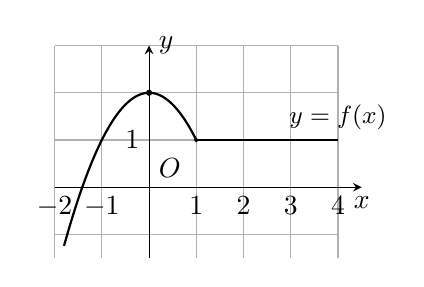
\begin{tikzpicture}[smooth,samples=300,scale=0.6,>=stealth]
			\draw[black!30!] (-2,-1.5) grid (4,3);
			\draw[->] (-2,0)--(4.5,0) node[below]{$x$};
			\draw[->] (0,-1.5)--(0,3) node[right]{$y$};
			\foreach \x in {-2,-1,1,2,3,4}{
				\draw (\x,0) node[below]{$\x$};%Ox
			}
			\foreach \y in {1}{
				\draw (0,\y) node[left]{$\y$};%Oy
			}
			\draw (0,0) node[above right]{$O$};
			\draw[domain=-1.8:1,thick] plot(\x,{-(\x)^2+2});
			\draw [thick](1,1)--(4,1) node[above]{\small $y=f(x)$};
			\draw[fill=black] (0,2) circle(1.5pt) (1,1) circle(1pt);
	\end{tikzpicture}}
	\loigiai{
		Quan sát đồ thị, ta có các kết quả $f(1)=1$, $f(3)=1$ và $f(4)=1$ nên
		$$P=2f(1)+f(4)-f(3)=2+1-1=2.$$
	}
\end{ex}

\begin{ex} Trong các công thức dưới đây, công thức nào được xem là công thức của một hàm số $y$ theo biến $x$?
	\choice
	{$3x^2-y^2=0$ }
	{\True $3x^2-y+1=0$}
	{$y^2=x$}
	{$(y-x)(y+x)=1$}
	\loigiai{
	}
\end{ex}
\begin{ex}%[0D2B1-4]
	Trong các đường biểu diễn dưới đây, đường nào \textbf{không} phải là đồ thị của một hàm số?
	\choice
	{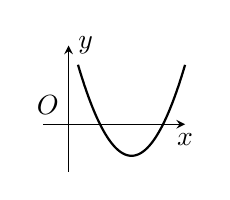
\begin{tikzpicture}[smooth,samples=300,scale=0.4,>=stealth]
		\draw[->] (-0.8,0)--(3.7,0) node[below]{$x$};
		\draw[->] (0,-1.5)--(0,2.5) node[right]{$y$};
		\draw (0,0) node[above left]{$O$};
		\draw[domain=0.3:3.7,thick] plot(\x,{(\x)^2-4*(\x)+3});
		\end{tikzpicture}}
	{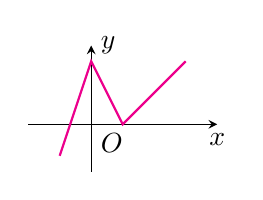
\begin{tikzpicture}[smooth,samples=300,scale=0.4,>=stealth]
		\draw[->] (-2,0)--(4,0) node[below]{$x$};
		\draw[->] (0,-1.5)--(0,2.5) node[right]{$y$};
		\draw (0,0) node[below right]{$O$};
		\draw[magenta,thick] (-1,-1)--(0,2)--(1,0)--(3,2);
		\end{tikzpicture}}
	{\True 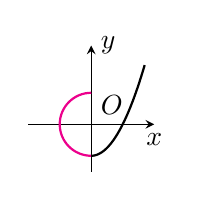
\begin{tikzpicture}[smooth,samples=300,scale=0.4,>=stealth]
		\draw[->] (-2,0)--(2,0) node[below]{$x$};
		\draw[->] (0,-1.5)--(0,2.5) node[right]{$y$};
		\draw (0,0) node[above right]{$O$};
		\draw[magenta,thick] (90:1) arc (90:270:1);
		\draw[domain=0:1.7,thick] plot(\x,{(\x)^2-1});
		\end{tikzpicture} }
	{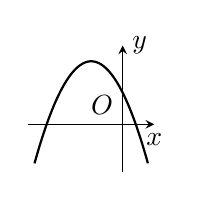
\begin{tikzpicture}[smooth,samples=300,scale=0.4,>=stealth]
		\draw[->] (-3,0)--(1,0) node[below]{$x$};
		\draw[->] (0,-1.5)--(0,2.5) node[right]{$y$};
		\draw (0,0) node[above left]{$O$};
		\draw[domain=-2.8:0.8,thick] plot(\x,{-(\x+3)^2+4*(\x+3)-2});
		\end{tikzpicture}}
	\loigiai{
	}
\end{ex}


\begin{ex}%[0D2B1-4]
	Trong các đường biểu diễn dưới đây, đường nào \textbf{không} phải là đồ thị của một hàm số?
	
	\choice
	{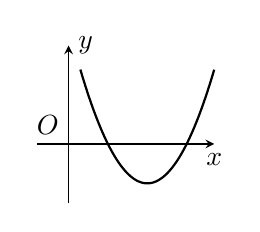
\begin{tikzpicture}[smooth,samples=300,scale=0.5,>=stealth]
			\draw[->] (-0.8,0)--(3.7,0) node[below]{$x$};
			\draw[->] (0,-1.5)--(0,2.5) node[right]{$y$};
			\draw (0,0) node[above left]{$O$};
			\draw[domain=0.3:3.7,thick] plot(\x,{(\x)^2-4*(\x)+3});
	\end{tikzpicture}}
	{\True 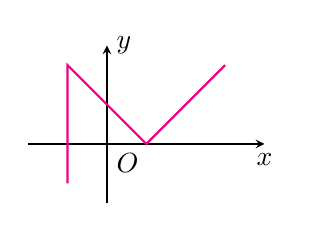
\begin{tikzpicture}[smooth,samples=300,scale=0.5,>=stealth]
			\draw[->] (-2,0)--(4,0) node[below]{$x$};
			\draw[->] (0,-1.5)--(0,2.5) node[right]{$y$};
			\draw (0,0) node[below right]{$O$};
			\draw[magenta,thick] (-1,-1)--(-1,2)--(1,0)--(3,2);
	\end{tikzpicture}}
	{ 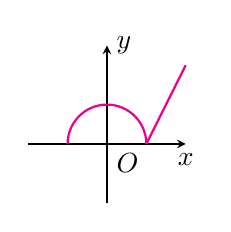
\begin{tikzpicture}[smooth,samples=300,scale=0.5,>=stealth]
			\draw[->] (-2,0)--(2,0) node[below]{$x$};
			\draw[->] (0,-1.5)--(0,2.5) node[right]{$y$};
			\draw (0,0) node[below right]{$O$};
			\draw[magenta,thick] (0:1) arc (0:180:1) (1,0)--(2,2);
		\end{tikzpicture} }
	{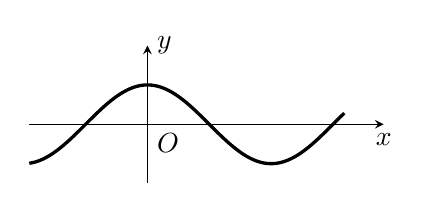
\begin{tikzpicture}[>=stealth,scale=0.5]
			\draw[->] (-3,0)-- (0,0) node [below right]{$O$}--(6,0) node[below]{$x$};
			\draw[->] (0,-1.5)--(0,2) node [right]{$y$};
			\draw [line width = 1.2pt, domain = -3:5, samples=150] plot (\x,{cos(\x*180/pi)});
			\end{tikzpicture}}
	\loigiai{
		}
\end{ex}

\begin{ex}
	Bảng giá cước gọi quốc tế của công ty viễn thông A được cho bởi bảng sau:
	\begin{center}
		\begin{tikzpicture}[xscale=7,yscale=0.8,font=\footnotesize]
			\begin{scope}[shift={(-.5,.5)}]
				\fill[orange!15] (0,-1) rectangle (1,-5);
				\fill[cyan!30] (0,0) rectangle (2,-1);
				\draw [line width=0.7pt,gray](0,0) grid (2,-5)
					;
			\end{scope}
			\path
			(0,0) node{\text{\textbf{Thời gian gọi (phút)}}}  
			(-0.4,-1) node[right]{Không quá 8 phút}
			(-0.4,-2) node[right]{Từ phút thứ 9 đến phút thứ 15}    
			(-0.4,-3) node[right]{Từ phút thứ 16 đến phút thứ 25}
			(-0.4,-4) node[right]{Từ phút 26 trở đi}    
					
			(1,0) node{\text{\textbf{Giá cước điện thoại (đồng/phút)}}}    
			(1,-1) node[right]{6500}
			(1,-2) node[right]{6000}    							
			(1,-3) node[right]{5500}
			(1,-4) node[right]{5000}    
				;
		\end{tikzpicture}
	\end{center}
	Ông An thực hiện cuộc gọi quốc tế 12 phút. Số tiền cước ông An phải trả là
	\choice
	{72 000 đồng  }
	{\True 76 000 đồng }
	{70 000 đồng }
	{90 000 đồng}
	\loigiai{
		\begin{itemize}
			\item [$\bullet$] Có thể thiệt lập biểu thức tính giá cước từ phút thứ 9 đến 15 là $6000t + 4000$. Thay $t =12$, ta được số tiền là 76 000 đồng.
			\item [$\bullet$] Hoặc tính nhanh: $ 8 \times 6500 + 4 \times 6000 = 76 000$ đồng.
		\end{itemize}
	}
\end{ex}
\begin{ex}%[0D2B1]
	Tìm tất cả các giá trị của $m$ để hàm số $y=\dfrac{x\sqrt{5}}{x^2-2x+m}$ có tập xác định là $\mathbb{R}$.
	\choice
	{\True $m>1$}
	{$m=1$}
	{$m<1$}
	{$m<0$}
	\loigiai{
	Hàm số có tập xác định là $\mathbb{R}$ khi và chỉ khi $x^2-2x+m =0$ vô nghiệm $\Leftrightarrow \Delta'=1-m<0 \Leftrightarrow m>1$.
	}
\end{ex}

\begin{ex}%[0D2G1-2]%
	Tìm các giá trị thực của tham số $m$ để hàm số $y=\dfrac{x+m+2}{x-m}$ xác định trên $(-1;2)$.
	\choice
	{$\left\{\begin{aligned}
			&m\leq -1\\
			&m\geq 2\\
		\end{aligned}\right. $}
	{$\left[\begin{aligned}
			&m<-1\\
			&m>2\\
		\end{aligned}\right. $ }
	{$-1<m<2$}
	{\True $\left[\begin{aligned}
			&m\leq -1\\
			&m\geq 2\\
		\end{aligned}\right. $ }
	\loigiai{
		Hàm số $y=\dfrac{x+m+2}{x-m}$ xác định khi $x\ne m$.\\
		Để hàm số $y=\dfrac{x+m+2}{x-m}$ xác định trên $(-1;2)$ khi và chỉ khi $\left[\begin{aligned}
			&m\leq -1\\
			&m\geq 2.\\
		\end{aligned}\right. $}
\end{ex}

\Closesolutionfile{ans}